\documentclass[11pt]{article}

\usepackage[margin=1.0in]{geometry}
\usepackage{tablefootnote}
\usepackage{graphicx}
\usepackage{natbib}
\usepackage{amsmath}
\usepackage{lscape}
\linespread{1.5}

\pdfminorversion 4

\bibpunct[,]{(}{)}{;}{a}{}{,}

\newcommand{\xline}[0]{\noindent\underline{\makebox[0.15cm][l]{}}}
\makeatletter
\def\hlinewd#1{%
	\noalign{\ifnum0=`}\fi\hrule \@height #1 \futurelet
	\reserved@a\@xhline}
\makeatother

\renewcommand{\bottomfraction}{.9}
\renewcommand{\topfraction}{.9}
\renewcommand{\textfraction}{0.1}
\renewcommand{\floatpagefraction}{.9}

%\usepackage{fancyhdr}

\begin{document}
	
\title{\textbf{The relationship between \emph{dN/dS} and scaled selection coefficients}}
\author{Stephanie J. Spielman$^{1*}$ and Claus O. Wilke$^{1}$}
\date{}

\maketitle
\noindent
Address:\\
$^1$Department of Integrative Biology, Center for Computational Biology and Bioinformatics, and Institute of Cellular and Molecular Biology.
The University of Texas at Austin, Austin, TX 78712, USA.\\

\bigskip
\noindent
$^*$Corresponding author\\
$\phantom{^*}$Email: stephanie.spielman@gmail.com\\
	
\bigskip
\noindent
Manuscript type: Article

\bigskip
\noindent Keywords: dN/dS, mutation-selection models, scaled selection coefficients, Markov models of sequence evolution

	
\newpage
\begin{abstract}
Numerous computational methods exist to assess the mode and strength of natural selection in protein-coding sequences, yet how distinct methods relate to one another remains entirely unknown. Here, we elucidate the relationship between two widely-used phylogenetic modeling frameworks: $dN/dS$ models and mutation-selection (MutSel) models. We derive a mathematical relationship between $dN/dS$ and scaled selection coefficients, the focal parameters of MutSel models, and use this relationship to gain deeper insight into the behaviors, limitations, and applicabilities of these two modeling frameworks. We prove that, if all synonymous changes are neutral, standard MutSel models correspond only to $dN/dS \leq 1$. However, if synonymous codons differ in fitness, $dN/dS$ can take on arbitrarily high values even if all selection is purifying. Thus, the MutSel modeling framework cannot necessarily accommodate positive, diversifying selection, while $dN/dS$ cannot distinguish between purifying selection on synonymous codons and positive selection on amino acids. We further propose a new benchmarking strategy of $dN/dS$ inferences against MutSel simulations and demonstrate that the widely-used Goldman-Yang-style $dN/dS$ models yield substantially biased $dN/dS$ estimates on realistic sequence data. By contrast, the less frequently used Muse-Gaut-style models display much less bias. Strikingly, the least-biased and most-precise $dN/dS$ estimates are never found in the models with the best fit to the data, measured through both AIC and BIC scores. Thus, selecting models based on goodness-of-fit criteria can yield poor parameter estimates if the models considered do not precisely correspond to the underlying mechanism that generated the data. In conclusion, establishing mathematical links among modeling frameworks represents a novel, powerful strategy to pinpoint previously unrecognized model limitations and strengths.
\end{abstract}



\section*{Introduction}
		
The oldest and most-widely used method to infer selection pressure in protein-coding genes calculates the evolutionary rate ratio $dN/dS$, which represents the ratio of non-synonymous to synonymous substitution rates. This metric indicates how quickly a protein's constituent amino acids change, relative to synonymous changes, and it is commonly used to identify protein sites that experience purifying selection ($dN/dS<1$), evolve neutrally ($dN/dS\approx1$), or experience positive, diversifying selection ($dN/dS>1$) \citep{NielsenYang1998, Yangetal2000, KosakovskyPondFrost2005b, Huelsenbecketal2006}. In phylogenetic contexts, $dN/dS$ is typically calculated using a maximum likelihood (ML) approach \citep{GoldmanYang1994,MuseGaut1994,NielsenYang1998,Yang2006}. ML methods assume a continuous time Markov model of sequence evolution, and since the introduction of Markov codon models in the 1990s, they have become a staple of comparative sequence analysis [see ref \citep{Anisimova2009} for a comprehensive review]. Throughout this paper, we will refer to these models as $dN/dS$-based models. 




A second class of Markov models, known as mutation-selection (MutSel) models, are increasingly being viewed as a viable alternative to the $dN/dS$ framework. While $dN/dS$-based models describe how quickly a protein's constituent amino acids change, MutSel models assess the strength of natural selection acting on specific mutations. Couched firmly in population-genetic theory, the MutSel framework estimates site-specific scaled selection coefficients $S=2N_es$, which indicate the extent to which natural selection favors, or disfavors, particular codon and/or amino acid changes \citep{HalpernBruno1998,YangNielsen2008,Rodrigueetal2010,Tamurietal2012}. Although first introduced over 15 years ago \citep{HalpernBruno1998}, MutSel models have seen little use due to their high computational expense. Recently, however, several computationally tractable model implementations have emerged \citep{RodrigueLartillot2014,Tamurietal2014}, allowing for the first time the potential for widespread adoption.		
		
Over the course of twenty years developement, $dN/dS$-based models have advanced to a high level of sophistication. These models can accommodate a variety of evolutionary scenarios, including synonymous rate variation \citep{MuseGaut1994,KosakovskyPondMuse2005} and episodic \citep{KosakovskyPondetal2011,MEME} and/or lineage-specific selection \citep{YangNielsen2002,Zhangetal2005,KosakovskyPondFrost2005a}, and they can also incorporate information regarding protein structure and epistatic interactions \citep{Robinsonetal2003,Thorneetal2007,Rodrigueetal2009,Scherreretal2012,MeyerWilke2013}. This flexibility, along with accessible software implementations \citep{KosakovskyPondetal2005,Yang2007,Delport2010}, makes $dN/dS$-based models an attractive analysis choice. On the other hand, some have argued that MutSel models, given their explicit basis in population-genetics theory and attention to site-specific amino-acid fitness differences, offer a more mechanistically realistic approach to studying coding-sequence evolution \citep{HalpernBruno1998,Rodrigueetal2010,Tamurietal2012,Thorne2012}. Moreover, a growing body of literature has demonstrated that $dN/dS$ estimates are particularly sensitive to violations in model assumptions, calling into question the general utility of $dN/dS$-based models \citep{Rochaetal2006,KryazhimskiyPlotkin2008,Ratnakumaretal2010,Mugaletal2014}.

Although both MutSel and $dN/dS$-based models describe the same fundamental process of coding-sequence evolution along a phylogeny, it is unknown how these two modeling frameworks relate to one another. In particular, as these inference methods have been developed independently, it remains an open question whether or not parameter estimates from one model are comparable to those of the other model. As a consequence, although certain rhetorical arguments may be made in favor of using one method over another, there is currently no formalized, concrete rationale to guide researchers in their methodological choices. Elucidating the relationship between these complementary modeling frameworks will more precisely reveal under which circumstances the use of these models is justified and has great potential to reveal previously unrecognized model behaviors, limitations, and capabilities.
		
Here, we formalize the relationship between these two modeling frameworks by examining the extent to which their respective focal parameters, $dN/dS$ and scaled selection coefficients, yield overlapping information about the evolutionary process. To this end, we derive a mathematical relationship between $dN/dS$ and scaled selection coefficients. We find that $dN/dS$ values can be precisely calculated from scaled selection coefficients, and that $dN/dS$ accurately captures the selective pressures indicated by a given distribution of scaled selection coefficients. Furthermore, we prove that, when synonymous mutations are neutral, it is only possible to recover $dN/dS \leq 1$ from selection coefficients, demonstrating that MutSel models, which commonly assume a static fitness landscape, are inherently only able to model purifying selection. Therefore, these models would be an inappropriate analysis method if positive selection is expected. However, we also find that, when synonymous codons have different fitnesses and hence purifying selection acts on synonymous changes, it is possible to recover $dN/dS$ values above 1, even though classical positive, diversifying selection is not occurring. Therefore, the $dN/dS$ framework cannot distinguish between positive, diversifying selection on amino acids and purifying selection on synonymous changes.

Finally, this relationship provides a uniquely rigorous platform to examine the performance of $dN/dS$-based models. Typically, researchers evaluate performance of a given inference framework through simulations that adhere to the underlying model's assumptions [but see refs.\ \citep{Schoniger1995, Mininetal2003, Holder2008, Yap2010, Rubinsteinetal2011}]. Indeed, simulated data is usually generated according to the same model as the inference framework, allowing for a direct comparison between the true and estimated parameter values. While this strategy is critical for testing whether a model implementation behaves as expected, it cannot assess model performance when the data are generated under a different process than the one modeled in the inference framework. However, in real-world sequence analysis, the inference framework will never exactly match the data-generation process. Therefore, a more sensitive test of model performance would examine how a given method performs when data are simulated under different mechanistic processes, and how sensitive the method is to violations of its assumptions. Unfortunately, such an approach is typically infeasible, because the relationships between parameters of interest among distinct model classes are generally not known.

The relationship we establish here between $dN/dS$ and selection coefficients allows us to overcome this limitation, as we can determine the true $dN/dS$ value directly from MutSel model parameters. Thus, we can assess performance of $dN/dS$-based inference frameworks by simulating data with a MutSel model and then comparing inferred $dN/dS$ ML estimates (MLEs) to $dN/dS$ values computed from selection coefficients. Using this strategy, we find, for sequences evolved under a symmetric mutation model, that $dN/dS$ values inferred in an ML framework agreed precisely with those calculated from scaled selection coefficients. However, as mutational asymmetry increases, $dN/dS$ MLEs become increasingly biased away from their true values, under a variety of ML model parameterizations. Surprisingly, the ML model parameterization which produced the most accurate $dN/dS$ estimates was never the model which exhibited the best fit to the data (measured by AIC and BIC), ultimately revealing that relying on model fit as a litmus-test for model performance can be an ineffective and misleading strategy. 

		
\section*{Results and Discussion}
		
		
\subsection*{Theoretical model}
This section contains a re-derivation of results presented in refs.\ \citep{HalpernBruno1998,YangNielsen2008}, reproduced here to introduce notation and to place the remainder of our work into context. We model sequence evolution using the Halpern-Bruno MutSel modeling framework under the assumptions of a fixed effective population size $N_e$ and constant selection pressure over time \citep{HalpernBruno1998,YangNielsen2008,Tamurietal2012,Thorne2012}.  This continuous-time reversible Markov process is governed by the $61 \times 61$ transition matrix $T(t) = e^{Qt}$, where the matrix $Q = q_{ij}$ gives the instantaneous substitution probabilities between all 61 sense codons, and diagonal elements of $Q$ satisfy $q_{ii} = -\sum_{i \neq j} q_{ij}$. We assume that only single-nucleotide substitutions occur instantaneously. 

Let $f^\text{codon}_i$ be the fitness of codon $i$, and let the selection coefficient acting on a mutation from codon $i$ to codon $j$ be $s_{ij} = f^\text{codon}_j - f^\text{codon}_i$ \citep{SellaHirsh2005,YangNielsen2008}. The fixation probability for this mutation is \citep{Kimura1962,HalpernBruno1998,YangNielsen2008}
\begin{equation}\label{eq:u_ij}
u_{ij} \approx \frac{2s_{ij}}{1 - e^{-2N_es_{ij}}} = \frac{1}{N_e}\frac{2N_es_{ij}}{1 - e^{-2N_es_{ij}}} .
\end{equation}
We further define $S_{ij} = 2N_es_{ij}$ (although note that this value would equal $4N_es_{ij}$ in diploids) as the scaled selection coefficient for this change \citep{YangNielsen2008}. The probability of a substitution from codon $i$ to $j$ is therefore
\begin{equation}\label{eq:q_ij}
q_{ij} = N_em_{ij}u_{ij} = m_{ij}\frac{S_{ij}}{1 - e^{-S_{ij}}} , 
\end{equation} where $m_{ij}$ is the codon mutation rate, which represents the rate at which codon $i$ transitions to codon $j$  \citep{HalpernBruno1998,SellaHirsh2005}. If we assume that $m_{ij}$ only has non-zero entries for  single-nucleotide changes, we can write it as $m_{ij}=\mu_{o_it_j}$, where $\mu_{kl}$ is the per-nucleotide mutation rate, $o_i$ is the origin (i.e., before mutation) nucleotide in codon $i$, and $t_j$ is the target (i.e., after mutation) nucleotide in codon $j$.

We now show how $S_{ij}$ can be written in terms of mutation rates and stationary (equilibrium) codon frequencies $P_i$. As this system satisfies detailed balance (reversibility) \citep{HalpernBruno1998,YangNielsen2008}, we have 
\begin{equation}\label{eq:DB}
q_{ij}P_i = q_{ji}P_j .
\end{equation} From equations \eqref{eq:q_ij} and \eqref{eq:DB}, we can write the ratio of substitution probabilities as 
\begin{equation}\label{ratio_q_ij}
\frac{P_i}{P_j} = \frac{m_{ji} S_{ji} (1-e^{-S_{ij}})} {m_{ij} S_{ij} (1-e^{-S_{ji}})} .
\end{equation} Using $S_{ij} = -S_{ji}$, we find that
\begin{equation}\label{eq:s_pmu}
S_{ij} = \ln\bigg{(} \frac{P_jm_{ji}}{P_im_{ij}} \bigg{)} .
\end{equation} This equation, previously derived in ref.\ \citet{HalpernBruno1998}, establishes a relationship between scaled selection coefficients and the stationary codon frequencies of the Markov chain. Moreover, in the specific case of symmetric mutation rates $m_{ij} = m_{ji}$, we have $S_{ij} = \ln\big{(}P_j/P_i\big{)}$ \citep{SellaHirsh2005}. 


		
\subsection*{Predicting \emph{dN/dS} from scaled selection coefficients} 

We now derive respective expressions for average nonsynonymous and synonymous evolutionary rates, which we can divide to obtain the evolutionary rate ratio $dN/dS$. We write the mean nonsynonymous rate $K_\text{N}$ as 
\begin{equation}\label{eq:KN}
	K_\text{N} = \sum_i \sum_{j \in {\cal N}_i} P_i q_{ij} \,,
\end{equation}
where ${\cal N}_i$ is the set of codons that are nonsynonymous to codon $i$ and differ from it by one nucleotide, and the substitution probability $q_{ij}$ is defined in equation \eqref{eq:q_ij}. To normalize $K_\text{N}$, we divide it by the number of nonsynonymous sites, which we calculate according to the mutational opportunity definition of a site \citep{GoldmanYang1994, Yang2006} as 
\begin{equation}\label{eq:LN}
	L_\text{N} = \sum_i \sum_{j \in {\cal N}_i} P_i m_{ij}\, .
\end{equation} Thus, we find that 
\begin{equation}\label{eq:dN}
	dN = \frac{K_\text{N}}{L_\text{N}}=\frac{\sum_i \sum_{j \in {\cal N}_i} P_i q_{ij}} {\sum_i \sum_{j \in {\cal N}_i}P_i m_{ij}}\,.
\end{equation} Similarly, for $dS$, the mean synonymous evolutionary rate $K_\text{S}$ per synonymous site $L_\text{S}$, we find
\begin{equation}\label{eq:dS}
	dS = \frac{K_\text{S}}{L_\text{S}}=\frac{\sum_i \sum_{j \in {\cal S}_i} P_i q_{ij} } {\sum_i \sum_{j \in {\cal S}_i} P_i m_{ij} }\,,
\end{equation}
where ${\cal S}_i$ is the set of codons that are synonymous to codon $i$ and differ from it by one nucleotide substitution. The quantities $K_\text{S}$ and $L_\text{S}$ are defined as in Eqs.~\eqref{eq:KN} and \eqref{eq:LN} but sum over $j\in {\cal S}_i$ instead of $j\in {\cal N}_i$. 

Moreover, under certain simplifying conditions, we can simplify the ratio given by equations \eqref{eq:dN} and \eqref{eq:dS} to a more intuitive form. 
If we assume symmetric mutation rates and that all synonymous codons have equal fitness (i.e.\ synonymous mutations are neutral), the synonymous fixation rate satisfies $u_{ij | j \in {\cal S}_i} = 1/N_e$ \citep{CrowKimura1970}, and hence the synonymous substitution probability becomes $q_{ij} = m_{ij}$. In this circumstance, the value for $dS$ reduces to 1, and the $dN/dS$ rate ratio reduces to the mean nonsynonymous substitution rate. If we further assume uniform mutation rates, $dN/dS$ becomes simply the average nonsyonymous fixation rate.

				
\subsection*{MutSel models specifically describe purifying selection}

We examined the relationship between $dN/dS$ and scaled selection coefficients by simulating 200 distributions of amino acid scaled fitness values, $F^\text{aa}_a = 2Nf^\text{aa}_a$, from a normal distribution $\mathcal{N}(0,\sigma^2)$. We drew a unique $\sigma^2$ for each fitness distribution from a uniform distribution $\mathcal{U}(0,4)$. Higher values for $\sigma^2$ correspond to larger fitness differences among amino acids, causing selection to act more strongly against nonsynonymous changes. Thus, high $\sigma^2$ values indicate strong purifying selection, low values indicate weak purifying selection, and $\sigma^2 = 0$ indicates that all amino acids are equally fit. We note that these $F^\text{aa}_a$ quantities correspond exactly to the amino-acid propensity parameters estimated by currently available site-specific MutSel inference methods \citep{RodrigueLartillot2014,Tamurietal2014}.

We then converted each amino-acid fitness distribution to a corresponding set of codon fitnesses, as described in \emph{Methods}. Briefly, for 100 of the distributions, we assumed that all synonymous codons had the same fitness, but for the other 100 distributions we allowed synonymous codons to have different fitnesses. In other words, the former 100 distributions do not incorporate purifying selection on synonymous changes whereas the latter 100 distributions do. Using equations \eqref{eq:KN} - \eqref{eq:dS}, we computed $dN/dS$ for each distribution of codon fitnesses. For these calculations, we assumed the symmetric mutation model HKY85 \citep{HKY85}, which is specified by the parameters $\mu$, the nucleotide mutation rate, and $\kappa$, the ratio of transitions to tranversions. Specifically, transitions occur at a rate $\mu\kappa$ and tranversions at a rate $\mu$. We used $\mu = 10^{-6}$ for all simulations, while we selected a unique value for $\kappa$ for each simulation from $\mathcal{U}(1,6)$.

Under neutral evolution, we expect that $dN/dS = 1$, and as purifying selection increases in strength, $dN/dS$ should correspondingly decrease. Therefore, we expect that $dN/dS$ will decline with the variance ($\sigma^2$) of the distribution of amino acid fitness values. Indeed, we observed a strong, negative correlation between these quantities (Figure~\ref{dnds_variance}). The larger the fitness differences among amino acids (higher $\sigma^2$), the lower $dN/dS$, properly reflecting increased purifying selection. This correlation was much stronger for fitness distributions without synonymous selection (Figure~\ref{dnds_variance}A) than for those with synonymous selection (Figure~\ref{dnds_variance}B). This difference emerged because fitness differences among synonymous codons obscured underlying amino-acid fitness differences. Even so, selection on synonymous codons did not negate the significant correlation between $dN/dS$ and overall selection strength.

Importantly, Figure~\ref{dnds_variance}A demonstrates that, in the limiting case when $\sigma^2$ approaches 0, and thus all codons have virtually the same fitness, $dN/dS$ converges to 1. In other words, when the protein-coding sequence evolved neutrally, selection coefficients correctly yielded a $dN/dS \approx 1$. Furthermore, we never recovered $dN/dS > 1$ when synonymous changes were neutral, revealing a key property of Halpern-Bruno style MutSel models: they inherently cannot describe positive, diversifying selection. Indeed, in Appendix 1, we prove that, under the assumptions that synonymous changes are neutral and mutation is symmetric, scaled selection coefficients strictly yield $dN/dS \leq 1$. This proof formalizes this MutSel model's underlying assumption that selection pressure is constant over the phylogeny and that the protein evolves under equilibrium conditions. Although this proof assumes symmetric mutation rates, we have found numerically that $dN/dS$ remains bounded from above by 1 even when mutations rates are asymmetric (Figure S1). 


\subsection*{Purifying selection on synonymous changes can produce \emph{dN/dS} $>1$}

The restriction $dN/dS \leq 1$ does not hold when synonymous changes are not neutral, as seen in Figure~\ref{dnds_variance}B. Wven though the Halpern-Bruno model explicitly assumes that the system is at equilibrium \citep{HalpernBruno1998,Thorne2012}, we find that $dN/dS$ can readily be greater than 1 under strong synonymous selection. In fact, it is theoretically possible to achieve arbitrarily high $dN/dS$ values when synonymous codon substitutions carry fitness changes. In the most extreme case of synonymous selection, where only a single codon per amino acid is selectively tolerated, the number of synonymous changes becomes $K_\text{S} = 0$, and thus the value for $dN/dS$ approaches infinity. Therefore, we find that $dN/dS > 1$ may indicate either positive, diversifying selection on amino acids or strong purifying selection on synonymous codons.

Given that the MutSel model framework assumes an overarching regime of purifying selection, this finding might seem paradoxical. However, the logical argument that $dN/dS > 1$ represents positive, diversifying selection assumes that the rate of synonymous change may be used as a neutral benchmark, an assumption clearly violated when selection acts on synonymous changes. Thus, the traditional signal of positive, diversifying selection, a $dN/dS$ value in excess of one, can result simply from strong synonymous fitness differences.

That sequences evolving under purifying selection can spuriously bear the hallmark of positive, diversifying selection highlights the pitfalls of naively interpreting $dN/dS$ values. Indeed, evolutionary constraints which induce synonymous selection are pervasive and affect virtually all domains of life \citep{GuZhouWilke2010}, from viruses \citep{Cuevasetal2011,ZaniniNeher2013} to plants \citep{Guetal2012} to Metazoa \citep{Duret2002,Chamaryetal2006,HershbergPetrov2008,PlotkinKudla2010,Lawrieetal2013}. 
Recent work has shown that synonymous rate variation is common across myriad proteins and contributes to evolutionary rate heterogeneity in up to 42\% of known protein families \citep{Dimitrieva2014}. For example, exonic splicing enhancers \citep{Schattner2006,Parmleyetal2006,ParmleyHurst2007}, regions contributing to mRNA secondary structure such as translation-initiation sites \citep{Chamaryetal2005,Schattner2006,GuZhouWilke2010,Cuevasetal2011,ZaniniNeher2013}, and DNA- and RNA-binding sites \citep{Parmleyetal2006} all experience moderate to strong synonymous selection. It has additionally been suggested that up to 18\% of mutational fitness effects in RNA viruses, whose genomes frequently feature sites with $dN/dS > 1$ \citep{Bushetal1999,Suzuki2006,Bhattetal2011,Meyeretal2013,MeyerWilke2013}, are caused by selection acting on synonymous changes \citep{Cuevasetal2011}. Finally, both selection against protein mis-folding and for translation efficiency tend to induce synonymous selection in a gene-specific manner \citep{WillifordDemuth2012,Agasheetal2013}, most notably in highly expressed genes \citep{DrummondWilke2008,Lawrieetal2013}. Therefore, while synonymous selection may not dominate genomes in organisms with relatively small effective population sizes \citep{Chamaryetal2006, PlotkinKudla2010}, it certainly acts strongly at specific sites and/or small, local regions. As $dN/dS$ ratios are typically measured on a per-site basis, we expect that some sites with $dN/dS > 1$ may in fact be false positives in the detection of positive, diversifying selection. We offer several approaches to ease this concern in \emph{Conclusions}.



\subsection*{Relationship between \emph{dN/dS} and scaled selection coefficients provides a novel benchmarking approach}

The relationship we have established between $dN/dS$ and scaled selection coefficients offers a unique opportunity to assess the robustness of $dN/dS$-based inference methods. It is conventional practice in model development to benchmark models against data simulated according to the model itself. While crucial for testing whether a given model has been correctly implemented, this strategy inherently cannot discern how the model behaves when data arose from a different mechanistic process. To overcome this limitation, we applied a novel benchmarking approach which used the theoretical relationship among modeling frameworks to assess the accuracy and specific utility of those models. Outlined in Figure~\ref{reg_conv}A, this approach entails comparing $dN/dS$ values calculated from selection coefficients to those inferred by a $dN/dS$-based model. Through this approach, we are able to simulate data which explicitly does not conform to the model used for inference, but we can still compare inferred parameter values to their true, simulated values using the relationship derived in the present work.

Using the selection coefficients and symmetric mutation rates from the previous two subsections, we simulated alignments using standard methods \citep{Yang2006} according to the Halpern-Bruno MutSel model \citep{HalpernBruno1998}. We then inferred a $dN/dS$ value for each alignment using the GY94 matrix \citep{GoldmanYang1994,NielsenYang1998}, which estimates $dN/dS$ with the parameter $\omega$. Throughout the remaining text, we refer to $dN/dS$ inferred using ML as $\omega$ or $\omega$ maximum likelihood estimate (MLE), and to $dN/dS$ computed using equations \eqref{eq:KN} - \eqref{eq:dS} simply as $dN/dS$. 

We found that $dN/dS$ values agree nearly perfectly with $\omega$ MLEs (Figure~\ref{reg_conv}B), and indeed this relationship was robust to both synonymous selection and uneven nucleotide composition (simulated alignments featured GC contents ranging from 0.21-0.89). Additionally, Figure~\ref{reg_conv}C demonstrates that $\omega$ converged to the true $dN/dS$ value as the size of the data set (i.e., simulated alignment length) increased. These results unequivocally show that, when nucleotide mutation is symmetric,  $dN/dS$-based model-inference methods behave exactly as expected, yielding precisely accurate $dN/dS$ estimates. This finding has important implications for modeling choices; although the MutSel framework might model the sequence evolution in a way that more mechanistically matches the evolutionary process, $dN/dS$-based models may suffice to model selective forces in phylogenetic data.


\subsection*{Biased \emph{dN/dS} estimates under asymmetric mutation models}
We next sought to test the accuracy of $dN/dS$-based models using more realistic parameter values. To this end, we determined codon fitness distributions from 498 unique distributions of experimentally-derived, site-specific amino-acid fitnesses for H3N2 influenza nucleoprotein (NP) \citep{Bloom2014a}. We combined each of these fitness distributions with three sets of experimentally-determined mutation rates, either for NP \citep{Bloom2014a}, yeast \citep{Zhu2014}, or polio virus \citep{Acevedo2014}, to determine $498 \times 3 = 1494$ distinct distributions of steady-state codon frequencies (see \emph{Methods} for details). While all three mutation matrices were asymmetric, each featured a differing degree of mutational bias; specifically, the mean ratios $\mu_{ij} / \mu_{ji}$ for NP, yeast, and polio mutation rates are 1.03, 1.69, and 5.25, respectively. For each resulting set of stationary codon frequencies, in combination with its respective set of mutation rates, we calculated $dN/dS$ and simulated alignments from which we inferred $\omega$. Note that we assumed no selection on synonymous codons for these calculations.

$dN/dS$-based model matrices account for nucleotide mutational bias by incorporating either target codon \citep{GoldmanYang1994} or target nucleotide \citep{MuseGaut1994} frequencies; these frameworks are known, respectively, as GY-style and MG-style models \citep{KosakovskyPond2010}. For example, the instantaneous rate matrix element giving the substitution probability from codon AAA to AAG would contain the target codon frequency $P_\text{AAG}$ in GY-style models but the target nucleotide frequency $\pi_\text{G}$ in MG-style models. Moreover, the GY-style models conform explicitly to a general-time reversible (GTR) form, whereas MG-style matrices do not, at first glance, appear to follow the same framework. However, as we show in Appendix 2, it is indeed posible to write MG-style matrices such that they conform to the GTR framework. This insight explicitly justifies using a time-reversible Markov process to describe these models, and it additionally demonstrates that the F1x4 codon frequency estimator \citep{MuseGaut1994} represents the state frequencies of the MG-style framework.

Previous works have suggested that MG-style and GY-style models yield different $\omega$ estimates \citep{KosakovskyPondMuse2005,Yap2010}, so we inferred $\omega$ according to both GY- and MG-style frameworks. For GY-style models, we used the frequency estimators F61 \citep{GoldmanYang1994}, F3x4 \citep{GoldmanYang1994}, CF3x4 \citep{KosakovskyPond2010}, and F1x4 \citep{MuseGaut1994}. For MG-style models, we considered both a parameterization with four global nucleotide frequency parameters and a parameterization which employed twelve nucleotide frequency parameters to allow for different frequencies at each codon position. We term the former framework MG1 and the latter MG3. Note that our MG1 corresponds to the original MG-style model \citep{MuseGaut1994}, whereas our MG3 corresponds to the so-called MG94$\times$HKY85 model \citep{KosakovskyPondMuse2005}. 

Figure~\ref{nyp_bias_r2} shows the resulting relationships between $dN/dS$ and $\omega$ MLEs for each set of mutation rates (NP, yeast, and polio), across model frequency parameterizations. Figure~\ref{nyp_bias_r2}A displays the estimator bias, defined as the average difference between the true $dN/dS$ value and the $\omega$ MLEs. Figure~\ref{nyp_bias_r2}B displays the precision in this relationship, measured by the squared correlation coefficient $r^2$ between $dN/dS$ and $\omega$. The exact bias and $r^2$ values are given in Tables S1 and S2, respectively, and full regression plots for $dN/dS$ vs.\ $\omega$ are shown in Figure S1.

Two distinct trends emerge from Figure~\ref{nyp_bias_r2}. First, asymmetry in the mutational process consistently induced significant bias in $\omega$ estimates. Most often, the model underestimated $\omega$ relative to the true $dN/dS$ value. Based on simulations without any selection ($dN/dS = 1$), ref.\ \citep{Yap2010} had previously suggested that GY-style models produce negatively biased $\omega$ estimates. Our results generalize this finding and show that this bias is pervasive, remains approximately constant through a wide range of $dN/dS$ values, and is not limited to the GY-style framework (Figure~\ref{nyp_bias_r2}A, Table S1, Figure S1). Furthermore, this bias systematically increased in magnitude as the underlying mutational process became more asymmetric. Indeed, for all frequency parameterizations, $\omega$ MLEs were most accurate under NP mutation rates, and both accuracy and precision tended to decrease as mutational bias progressed from yeast to polio mutation rates. 

Second, frequency parameterizations which more closely matched the mechanistic process that generated the data (MG1 and MG3) generally outperformed all other frequency estimators. In particular, MG1 clearly performed the best of all frequency estimators considered, featuring by far the least amount of estimator bias for the highly asymmetric polio mutation rates. This result makes intuitive sense, as the MG-style framework most mechanistically matches the MutSel framework among all $dN/dS$-based frameworks examined here. Indeed, in the case of neutral evolution, $\omega = 1$ in an MG-style matrix, and the ratio of fixation probabilities in the MutSel matrix will also equal 1. Therefore, nucleotide mutation rates alone comprise each model's rate matrix, demonstrating that MG-style and MutSel models are virtually identical under neutral evolution. Importantly, this correspondence does not hold for GY-style matrices which, as they incorporate target codon frequencies, do not explicitly consider nucleotide mutation rates. Thus, we highly recommend that researchers employ MG-style matrices in their $dN/dS$ inferences to minimize bias (we note that this modeling framework is available through HyPhy \citep{KosakovskyPondetal2005} and/or the Datamonkey server \citep{Delport2010}).


\subsection*{Model with best fit is not the model that yields the most accurate parameter estimates}

Strikingly, when we examined model fit using AIC scores \citep{Akaike1974,BurnhamAnderson2004} for the different frequency parameterizations, we found that the F61 parameterization was unequivocally the best-performing model, on average, for all datasets (Table~\ref{tab:dAIC}). This result dramatically juxtaposed the substantial inaccuracy and imprecision in $\omega$ that F61 frequently yielded. In particular, F61 had the most estimator bias for NP datasets as well as the least precision for both NP and polio datasets (Figure~\ref{nyp_bias_r2}). Thus, we found AIC could not identify the model which produced the most accurate estimates for the parameter of interest. 

Although this result may seem counterintuitive, it is important to note that AIC measures goodness-of-fit by approximating the Kullback-Leibler (KL) distance between a given candidate model and the true model. As the MutSel framework defines selection coefficients in terms of stationary frequencies, it indeed follows that the F61 estimator, which explicitly incorporates empirical codon frequencies into the rate matrix, should be selected as the best-fitting model, in spite of its biased parameter estimates. Therefore, we additionally assessed whether BIC might provide a more accurate indication of model performance. However, BIC scores yielded the same overarching trend as did AIC scores in which F61 dramatically outperformed all other frequency parameterizations (Table S3).

This finding has broad implications for practices in model selection. In particular, it appears that model fit can be confounded with model accuracy, such that the model with better model fit may produce less accurate parameter estimates. We find that, if the data are generated by a process distinct from the inference model, standard model selection quantities cannot necessarily identify which model produces the most precise and least biased parameter estimates. Good model fit, therefore, may not have any bearing on whether using that model is mechanistically justified, and selecting models based solely on fit may not guard effectively against spurious inferences but instead prove misleading. We suggest that the mechanism producing the data should be carefully considered, and an appropriate inference method which best approximates this process should then be selected. 

Finally, these results provide a concrete example of previous theoretical suggestions that AIC might fail in phylogenetic model selection \citep{Liberles2013}. Indeed, previous work has suggested that Bayes Factors might serve as a better indication of model performance than AIC, albeit results were obtained in a Bayesian rather than frequentist framework \citep{Rodrigue2008}. Therefore, it is clear further investigation into the performance of various model fit criteria for complex models is strongly warranted. 



\section*{Conclusions}
By elucidating the relationship between $dN/dS$ and scaled selection coefficients, we have shown that $dN/dS$-based and MutSel models convey consistent information regarding the strength of natural selection. Importantly, our proof that $dN/dS \leq 1$ (assuming symmetric mutation and no synonymous selection) indicates that the use of the Halpern-Bruno MutSel modeling framework is only justified under purifying selection. This restriction is in part indicated by this model's assumption of constant selection pressures over time, or in other words a static fitness landscape \citep{HalpernBruno1998,Thorneetal2007,Rodrigueetal2010,Thorne2012}. Thus, if the aim is to identify positive, diversifying selection, of the two frameworks examined here, only $dN/dS$-based models are appropriate. However, different MutSel frameworks not examined here that allow fitnesses to fluctuate over time should serve as a promising avenue for future research extending the applicability of this modeling framework \citep{Whelan2008,MustonenLassig2009}.

However, we have also found that $dN/dS$ values can readily be greater than 1 when selection acts on synonymous mutations, even though the protein sequence is evolving solely under purifying selection. This seemingly paradoxical finding actually reflects an assumption violation; the assertion that $dN/dS > 1$ necessarily corresponds to positive, diversifying selection requires that synonymous changes are neutral, which clearly does not hold if there are fitness differences among synonymous codons. This result contributes to a growing body of literature which has found that purifying selection can yield $dN/dS > 1$ if model assumptions are not met. For instance, $dN/dS$ can be greater than 1, even under purifying selection, if sequences contain segregating polymorphisms \citep{Rochaetal2006,KryazhimskiyPlotkin2008,Mugaletal2014} or when GC-biased gene conversion is pervasive \citep{Ratnakumaretal2010}. Thus, it is becoming increasingly clear that the $dN/dS = 1$ neutral threshold typically used to distinguish purifying and positive selection is highly sensitive to violations in model assumptions. We emphasize that it is crucial to verify that data adhere to model assumptions before conclusions from $dN/dS$ are drawn.

We suggest several strategies to limit such false positive results under synonymous selection. For one, certain formulations of $dN/dS$-based methods consider $dN$ and $dS$ rate variation separately \citep{MuseGaut1994,KosakovskyPondMuse2005,Mayroseetal2007,Murrell2013} rather than using a single parameter to represent $dN/dS$. These kinds of methods, and indeed others which explicitly model nucleotide-level selection in conjunction with codon-level selection \citep{Rubinsteinetal2011} or correct $dS$ for synonymous selection \citep{Zhouetal2010}, may be able to distinguish situations in which $dN/dS>1$ because $dN$ is unusually large (positive selection) or $dS$ is unusually small (purifying selection). Finally, our benchmarking approach, in which we simulate sequences according to MutSel models and infer $dN/dS$ both from MutSel parameters directly and using ML, may be used to benchmark these kinds of models and may help to identify circumstances under which synonymous selection confounds $dN/dS$ interpretations. 

Finally, we emphasize the utility of establishing relationships among distinct modeling frameworks to probe model behavior and evaluate model performance. Such an approach is uniquely able to reveal unrecognized behaviors and/or limitations of different modeling frameworks and can precisely reveal the circumstances in which different models are best suited. We hope that further studies in this spirit will ensure robust model development in future studies.


\section*{Methods}

\subsection*{Simulation of scaled selection coefficients}

To examine the relationship between $dN/dS$ and scaled selection coefficients, we simulated 200 distributions of amino-acid scaled fitness values, $F^\text{aa}_a = 2Nf^\text{aa}_a$, from a normal distribution $\mathcal{N}(0,\sigma^2)$, where a unique $\sigma^2$ for each fitness distribution was drawn from a uniform distribution $\mathcal{U}(0,4)$. We converted these amino-acid fitnesses to codon fitnesses as follows. For 100 of the fitness distributions, we directly assigned all codons within a given amino acid family the fitness $F^\text{codon}_i = F^\text{aa}_a$, so that all synonymous codons had the same fitness. For the other 100 fitness distributions, we assigned synonymous codons different fitnesses by randomly drawing a preferred codon for each amino acid. This preferred codon was assigned the fitness of $F^\text{codon}_i = F^\text{aa}_a + \lambda$, and all non-preferred codons were given the fitness $F^\text{codon}_j = F^\text{aa}_a - \lambda$. We drew a unique $\lambda$ for each fitness distribution from $\mathcal{U}(0,2)$. 
We then computed stationary codon frequencies as 
\begin{equation}\label{eq:boltzmann}
P_i = \frac{e^{F^\text{codon}_i}}{\sum_k e^{F^\text{codon}_k}}, 
\end{equation} where the sum in the denominator runs over all 61 sense codons \citep{SellaHirsh2005}. Equation \eqref{eq:boltzmann} gives the analytically precise stationary frequencies for a MutSel model, under the assumption of symmetric mutation rates \citep{SellaHirsh2005}. We used equations \eqref{eq:KN} - \eqref{eq:dS} to compute $dN/dS$ for each resulting set of stationary codon frequencies. For these calculations, we assumed the HKY85 \citep{HKY85} nucleotide mutation model, and accordingly we set the transition mutation rate as $\mu\kappa$ and the transversion rate as $\mu$. We used the value $\mu = 10^{-6}$ for all $dN/dS$ calculations, and we drew a unique value for $\kappa$ from $\mathcal{U}(1,6)$ for each set of codon frequencies.


\subsection*{Alignment simulations}
We simulated protein-coding sequences as a continuous-time Markov process using standard methods \citep{Yang2006} according to the Halpern-Bruno MutSel model \citep{HalpernBruno1998}. In brief, this model's instantaneous rate matrix $Q = q_{ij}$ is populated by elements
\begin{equation}\label{eq:HBmatrix}
q_{ij} = \left\{ 
\begin{array}{rl}
m_{ij} \frac{S_{ij}}{1-1/S_{ij}} &\text{single nucleotide change} \\\\
0                                  &\text{multiple nucleotide changes} \\             
\end{array} \right.,
\end{equation} for a mutation from codon $i$ to $j$, where $m_{ij}$ is the mutation rate, and the scaled selection coefficient $S_{ij}$ is defined in equation \eqref{eq:s_pmu}. All alignments presented here were simulated along a symmetric 4-taxon phylogeny with all branch lengths equal to 0.01, beginning with a root sequence generated in proportion to  stationary codon frequencies \citep{Yang2006}. Unless otherwise stated, all simulated alignments contained 500,000 codon positions. A single evolutionary model was applied to all positions in the simulated sequences. While this lack of site-wise heterogeneity is unrealistic for real sequence evolution, it allowed us to verify our derived relationship between scaled selection coefficients and $dN/dS$ with a sufficiently sized data set. 

\subsection*{Computation of stationary frequencies for experimental data sets}
We used experimentally-determined site-specific amino-acid fitness parameters $F^\text{aa}_a$ for influenza nucleoprotein (NP), from ref.\ \citep{Bloom2014a}, in combination with experimental nucleotide mutation rates for either NP \citep{Bloom2014a}, yeast \citep{Zhu2014}, or polio virus \citep{Acevedo2014}, to derive realistic distributions of stationary codon frequencies. We combined each of the  498 site-wise amino-acid preference sets reported by ref.\ \citep{Bloom2014a} with each of the three mutation-rate matrices to construct a total of $498 \times 3 = 1494$ unique experimental evolutionary Markov models, using the approach in refs.\ \citep{Bloom2014a,Bloom2014b}. The instantaneous rate matrix $Q$ for each experimental model is populated by elements
\begin{equation}
q_{ij} =  \left\{ 
\begin{array}{rl}
  \text{max}(1, F^\text{codon}_j \big{/} F^\text{codon}_i)m_{ij} & \text{single nucleotide change} \\
  0                                                & \text{multiple nucleotide changes}  \\
\end{array} \right.
\end{equation} for a substitution from codon $i$ to codon $j$, where $F^\text{codon}_i$ is the fitness of codon $i$ \citep{Bloom2014a,Bloom2014b}. We calculated $F^\text{codon}_i$ values by simply assigning a given amino acid's experimental fitness $F^\text{aa}_a$ to each of its constituent codons; thus, all synonymous changes were neutral. We determined the stationary codon frequencies for each resulting experimental model from the matrix's eigenvector corresponding to the eigenvalue 0. Finally, we simulated alignments for each set of stationary frequencies and corresponding mutation rates according to the Halpern-Bruno model (equation \eqref{eq:HBmatrix}).   

		
\subsection*{Maximum likelihood inference of \emph{dN/dS}}
For the 200 alignments simulated with symmetric mutation rates, we inferred $dN/dS$ using the M0 model \citep{Yangetal2000}, as implemented in the HyPhy batch language \citep{KosakovskyPondetal2005}. The M0 model uses the GY94 instantaneous rate matrix, which is populated by elements
\begin{equation}\label{eq:GY94}
q_{ij} = \left\{ 
	\begin{array}{rl}
	P_j                &\text{synonymous transversion} \\
	\kappa P_j           &\text{synonymous transition} \\
 	\omega P_j           &\text{nonsynonymous transversion} \\
 	\omega \kappa P_j    &\text{nonsynonymous transition} \\
	0                    &\text{multiple nucleotide changes} \\             
	\end{array} \right.,
\end{equation} for a substitution from codon $i$ to codon $j$, where $\kappa$ is the transition-transversion bias, $P_j$ is the equilibrium frequency of the target codon $j$, and $\omega$ represents $dN/dS$ \citep{GoldmanYang1994,NielsenYang1998}. The $P_i$ parameters are intended to represent those codon frequencies which would exist in absence of selection pressure generated by mutation alone \citep{GoldmanYang1994,MuseGaut1994,YN00,Yang2006}. Thus, when inferring $\omega$ on datasets which used symmetric mutation rates, we assigned the value $1/61$ to all parameters $P_i$, as all codons are equally probable under unbiased mutation.

Alternatively, when inferring $\omega$ for alignments simulated with experimental fitness and mutation rates, we used several different model parameterizations, including GY-style \citep{GoldmanYang1994} (target codon frequency) and MG-style \citep{MuseGaut1994} (target nucleotide frequency) parameterizations. We considered the GY-style parameterizations F61 \citep{GoldmanYang1994}, F3x4 \citep{GoldmanYang1994}, CF3x4 \citep{KosakovskyPond2010}, and F1x4 \citep{MuseGaut1994}. We implemented two varieties of MG-style models; the first, MG1, employs four parameters for nucleotide frequencies (one per nucleotide) \citep{MuseGaut1994}, and the second, MG3, employs twelve nucleotide frequency parameters, with four nucleotide frequency parameters for each of the three codon positions \citep{KosakovskyPondMuse2005}. All frequency parameters were estimated from the data. Note that we used the state frequencies of F1x4 for the MG1 framework and F3x4 for the MG3 framework. In addition to frequency parameter, all models included the parameters $\kappa$ and $\omega$.

\subsection*{Availability}
All code is freely available from \\ \texttt{https://github.com/clauswilke/Omega\_MutSel}. Alignments were simulated using the sequence simulation library pyvolve, available from  \\ \texttt{https://github.com/sjspielman/pyvolve}. Simulated alignments are available from Dryad at doi:XXX (data will be submitted upon acceptance of this article).



\section*{Appendix 1}
We prove that $dN/dS \leq 1$ when calculated from scaled selection coefficients. We assume that mutation rates are symmetric ($m_{ij} = m_{ji}$) and that synonymous codons have the same fitness (synonymous changes are neutral). As described in the main text, these assumptions yield $dS = 1$, and hence we have to show that $dN = K_\text{N}\big{/}L_\text{N} \leq 1$. To this end, we note that the sums in $K_\text{N}$ and $L_\text{N}$ can be reordered such that the substitution probability from codon $i$ to $j$ is always added to the substitution probability from codon $j$ to $i$. We can then show that the sum of each of these pairs in the expression for $K_\text{N}$ is smaller than the corresponding term in $L_\text{N}$, and hence $dN/dS \leq 1$.

Without loss of generality, we consider a pair of nonsynonymous codons $i$ and $j$ whose respective stationary frequencies $P_i$ and $P_j$ satisfy $P_i \leq P_j$ and $P_i, P_j \geq 0$. As follows from equations \eqref{eq:q_ij} and \eqref{eq:s_pmu}, the sum of the probability weights of evolving from codon $i$ to $j$ and from codon $j$ to $i$ is
\begin{equation}
N_em_{ij} u_{ij} + N_em_{ji} u_{ji}  = \frac{2P_iP_j[\log(P_i) - \log(P_j)]}{P_i - P_j} \,.
\end{equation}
This quantity represents $K_\text{N}$ in the $dN$ calculation. To prove $dN \leq 1$, we must show that this quantity is less than or equal to $P_i + P_j$, which represents $L_\text{N}$ in the $dN$ calculation. To this end, we introduce the function 
\begin{equation}\label{eq:Fxy}
F(x,y) = x + y - \frac{2xy[\log(x) - \log(y)]}{x - y} \,,
\end{equation}
and we will now show that $F(x,y) \geq 0$ for $x \leq y$ and $y \geq 0 $. Using l'H\^{o}pital's rule, it is straightforward to show that $\lim_{|x - y| \to 0}F(x,y) = 0$, which can in turn be extended to hold under the condition $x=y$. For $x < y$, we show that the first derivative of equation \eqref{eq:Fxy} is negative throughout $x \in (0,y)$, which proves that the function monotonically decreases, and thus $F(x,y) > 0$, in this interval. We calculate the first derivative as 
\begin{equation}
\frac{\partial{F(x,y)}}{\partial{x}} = \frac{\big{[} (x-3y)(x-y) - 2y^2(\log{x} - \log{y}) \big{]}}{(x-y)^2} \,.
\end{equation}
We now replace the expression $\log{x} - \log{y}$ by its Taylor series expansion, yielding
\begin{equation}\label{eq:expand}
	\frac{\partial{F(x,y)}}{\partial{x}} = 
	\frac{ \bigg{[} (x-3y)(x-y) - 2y^2\bigg{(}\sum\limits_{n=1}^\infty \frac{1}{n} (1-x/y)^n\bigg{)} \bigg{]}}{(x-y)^2} \,.
\end{equation} We note that the first two terms of the Taylor series equal $(x-3y)(x-y)$, and thus expression \eqref{eq:expand} simplifies to 
\begin{equation}
\frac{\partial{F(x,y)}}{\partial{x}} = \frac{-2y^2\sum\limits_{n=3}^\infty \frac{1}{n} \big{(}1-\frac{x}{y}\big{)}^n}{(x-y)^2} ,
\end{equation}
which is clearly negative. This concludes the proof.


\bigskip



\section*{Appendix 2}
GY-style matrices may be expressed in the framework of the general-time reversible (GTR) model, in which the instantaneous matrix $Q$ can be decomposed into a $61 \times 61$ symmetric substitution rate matrix and a 61-dimensional vector containing the equilibrium codon frequencies. The latter corresponds to the stationary distribution of the Markov chain. By contrast, MG-style rate matrices are written in terms of nucleotide frequencies rather than codon frequencies. Therefore, whether these models fit into the GTR framework is unclear \emph{a priori}. We now describe how the MG-style matrix can be rewritten in terms of a symmetric matrix and a vector of equilibrium codon frequencies, thus demonstrating that these matrices also fit into the GTR framework.
 
MG-style matrix elements, for a the substitution from codon $i$ to $j$, are generally given by 
\begin{equation}\label{eq:MGstyle}
q_{ij} = \left\{ 
\begin{array}{rl}
\theta_{o_it_j}\pi_{t_j}          &\text{synonymous change} \\
\omega \theta_{o_it_j}\pi_{t_j}   &\text{nonsynonymous change} \\
0                             &\text{multiple nucleotide changes}       
\end{array} \right. ,
\end{equation} where $\omega$ is the ratio of nonsynonymous to synonymous substitution rates and the product $\theta_{o_it_j}\pi_{t_j}$ corresponds to a nucleotide-level mutation rate $\mu_{o_it_j}$, where $o_i$ is the origin nucleotide in codon $i$, and $t_j$ is the target nucleotide in codon $j$. Note that the matrix $\theta_{o_it_j}$ is symmetric in $o_i$ and $t_j$.

For a given codon $i$, the matrix of Eq.\ \eqref{eq:MGstyle} yields the stationary frequency $P_i = \pi_{i_1}\pi_{i_2}\pi_{i_3}C$, where $C = 1 - \Pi_\text{stop}$ and $\Pi_\text{stop} = \pi_\text{T}\pi_\text{A}\pi_\text{G} + \pi_\text{T}\pi_\text{G}\pi_\text{A} + \pi_\text{T}\pi_\text{A}\pi_\text{A}$ \citep{MuseGaut1994}. Therefore, we can rewrite the term $\theta_{o_it_j}\pi_{t_j}$ as $\theta_{o_it_j}P_jC / (\pi_m\pi_n)$, where $m$ and $n$ are the nucleotides which do not change in a given instantaneous codon substitution. This allows us to rewrite the rate instantaneous matrix as 
\begin{equation}
q_{ij} = \left\{ 
\begin{array}{rl}
\frac{C\theta_{o_it_j}}{\pi_m\pi_n} P_j           &\text{synonymous change from $i$ to $j$} \\\\
\omega\frac{C\theta_{o_it_j}}{\pi_m\pi_n} P_j     &\text{nonsynonymous change from $i$ to $j$} \\\\
0                                              &\text{multiple nucleotide changes} \\           
\end{array} \right.
\end{equation} for a substitution from codon $i$ to codon $j$, and this matrix clearly conforms to the GTR framework.
		
\section*{Acknowledgements}
This work was supported in part by NIH grant R01 GM088344, ARO grant W911NF-12-1-0390, DTRA grant HDTRA1-12-C-0007, and NSF Cooperative Agreement No. DBI-0939454 (BEACON Center).  Computational resources were provided by the University of Texas at Austin's Center for Computational Biology and Bioinformatics (CCBB).

		
		
\bibliographystyle{MBE}
\bibliography{bibliography}
		
	
	
\section*{Figures and Tables}

\vspace{2cm}
	
\begin{figure}[htbp]
	\centerline{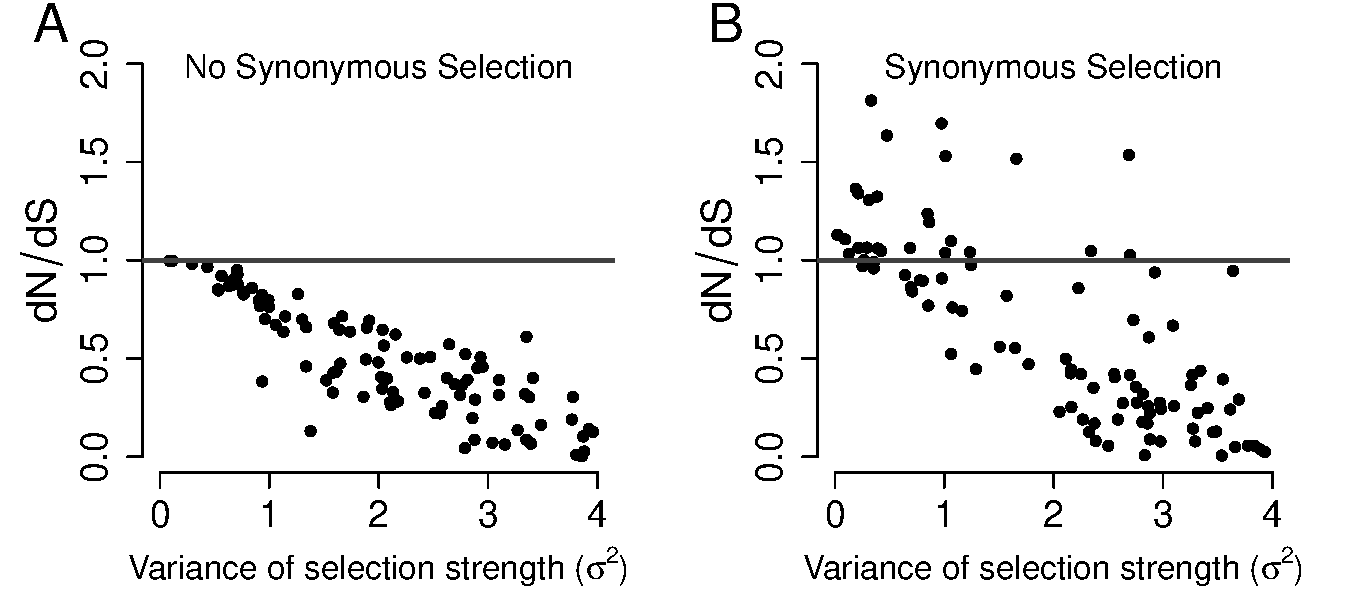
\includegraphics[width=12cm]{figures/MainText/dnds_variance.pdf}}
	\caption{\label{dnds_variance} $dN/dS$ decreases in proportion to amino-acid level selection strength. $dN/dS$ is plotted against the variance ($\sigma^2$) of the simulated distribution of amino-acid scaled fitness values. Higher variances indicate larger fitness differences among amino acids, whereas the limiting value of $\sigma^2 = 0$ indicates that all amino acids have the same fitness. (A) Synonymous codons have equal fitness values ($r^2=0.83, P < 2^{-16}$). (B) Synonymous codons have different fitness values ($r^2=0.45, P < 2^{-16}$). Note that panel B, but not A, shows $dN/dS$ values greater than 1, in spite of the steady-state evolutionary process. In each panel, the dashed line indicates the $y=1$ line, and the solid line indicates the regression line.}
\end{figure}
		
		
\vspace{2cm}
		
\begin{figure}[htbp]
	\centerline{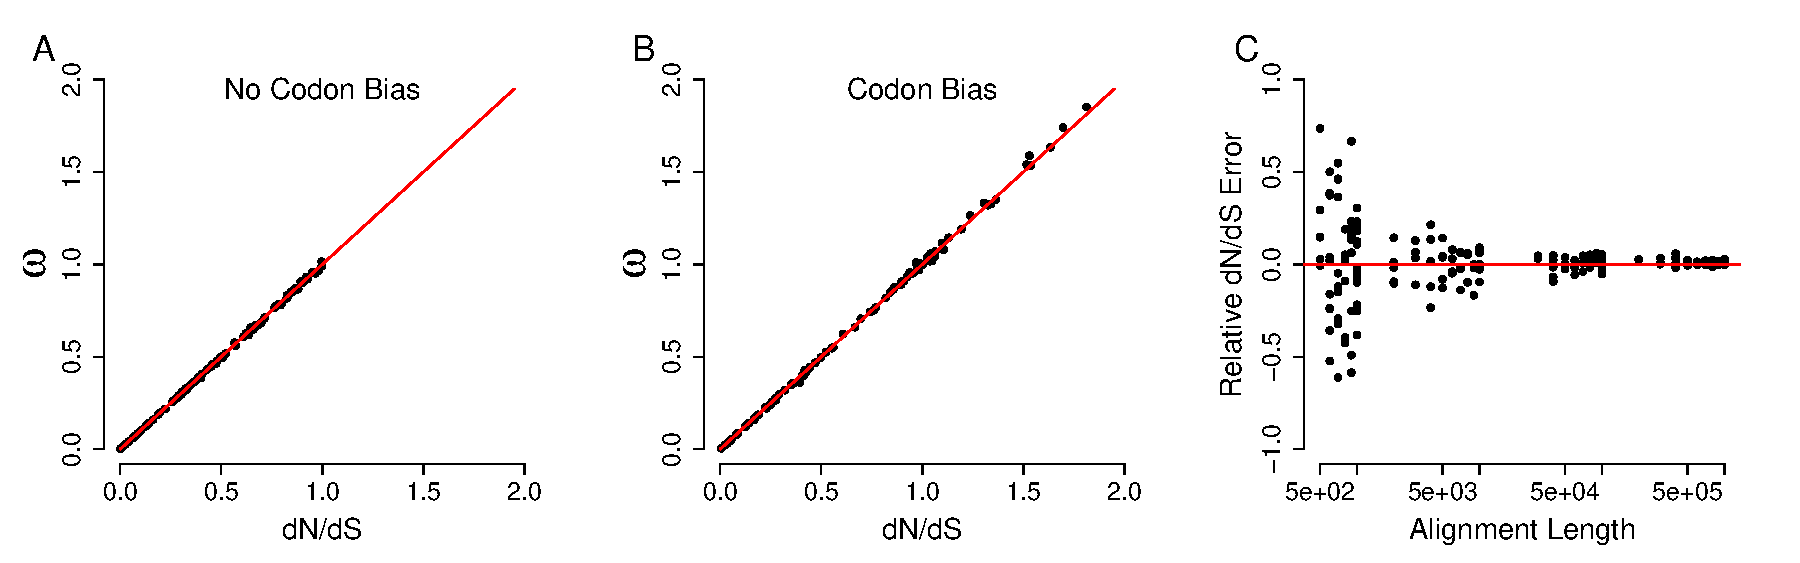
\includegraphics[width=12cm]{figures/MainText/regression_convergence.pdf}}
	\caption{\label{reg_conv} Combined modeling approach to assess performance of $dN/dS$ inference frameworks. (A) Protein-coding alignments are simulated in the MutSel modeling framework. $dN/dS$ can then be calculated (``predict") from scaled selection coefficients as well as through an ML inference framework (``infer"). Comparing resulting quantities reveals the accuracy of the chosen inference framework. (B) Regression between predicted $dN/dS$ values and inferred $\omega$ MLEs. Each point corresponds to a single simulated alignment, and the solid line is the $x=y$ line. (C) Convergence of $\omega$ MLEs to the true $dN/dS$ value. The y-axis indicates the relative error of the $\omega$ MLE, and the x-axis indicates the number of positions in the simulated alignment. As the number of positions and hence the size of the data set increases, $\omega$ converges to the predicted $dN/dS$ value. The solid line is the $y=0$ line, indicating no error.}
\end{figure}
	
\vspace{2cm}
	

\begin{figure}[htbp]
	\centerline{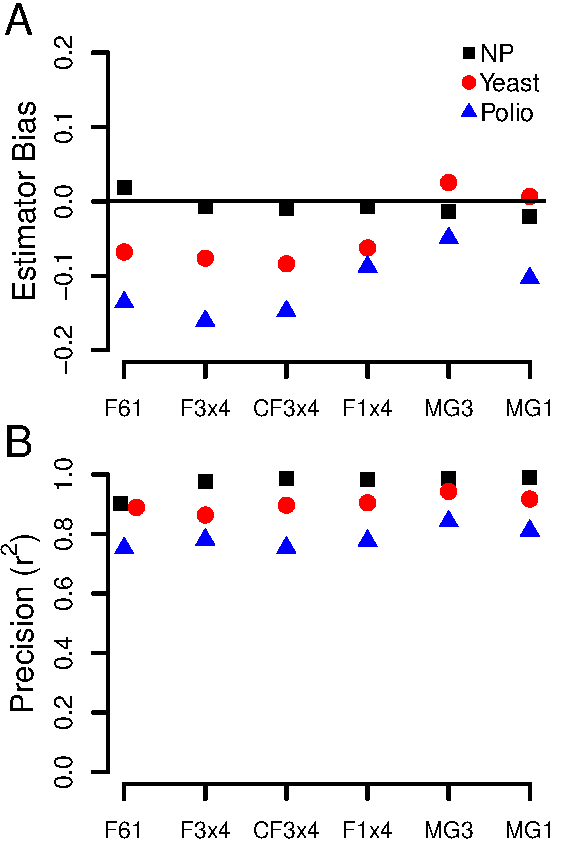
\includegraphics[width=12cm]{figures/MainText/nyp_bias_r2.pdf}}
	\caption{\label{nyp_bias_r2} Estimator bias and precision of $\omega$ estimates for various model frequency parameterizations. (A) Estimator bias and (B) Precision ($r^2$) values between $dN/dS$ and $\omega$ MLEs across model frequency parameterizations, for each set of nucleotide mutation rates. To calculate bias, we fit a linear model with $\omega$ as the response and $dN/dS$ as the predictor, with a fixed slope of 1, and the resulting intercept value represents the bias. Negative biases indicate $\omega$ MLEs that are, on average, lower than $dN/dS$. Note that all standard errors for bias are smaller than the symbol size.}	
\end{figure}

\vspace{2cm}


\begin{table}[htbp]
	\caption {\label{tab:dAIC} Mean $\Delta$AIC for datasets simulated with NP, yeast, or polio virus mutation rates.}
	\begin{tabular}{l c c c}
		\hline\noalign{\smallskip}
		\multicolumn{1}{c}{Frequencies} & NP & Yeast & Polio \\
		\noalign{\smallskip}\hline\noalign{\smallskip}
              F61 & 0 & 0 & 0 \\ 
              CF3x4 & -9519.53 & -7843.77 & -7975.94 \\ 
              MG1 & -13207.5 & -9924.05 & -5147.57 \\ 
              F1x4 & -13410.54 & -13544.47 & -15468.29 \\ 
              MG3 & -14287.28 & -12737.57 & -8624.87 \\ 
              F3x4 & -14699.22 & -17277.3 & -19384.58 \\ 
		\noalign{\smallskip}\hline\noalign{\smallskip} 	
	\end{tabular}

\noindent {\footnotesize \textbf{Note:} The order of frequency models shown in the table corresponds to the model ranking for NP, and the ranking differs somewhat for yeast and polio datasets. AIC is computed as $AIC = 2(k - \ln L)$, where $k$ is the number of free parameters of the model, and $\ln L$ is the log-likelihood \citep{Akaike1974,BurnhamAnderson2004}. Number of free parameters for each model is F61, 63; CF3x4, 12; MG1, 6; F1x4, 6; MG3, 12; and F3x4, 12. Note that, for each model, 3 of the parameters are $\omega$, $\kappa$, and a global branch-length scaling parameter, and the remaining parameters are either empirical codon or nucleotide frequencies.}
\end{table}


\clearpage

	
\section*{Supplementary Information}

\vspace{2cm}

\noindent Table S1. Estimator bias of $\omega$ MLEs and the true $dN/dS$ values, for all nucleotide mutation rates and model frequency parameterizations examined. All biases are statistically significant (different from 0), with all $P < 2\times10^{-16}$ except for the estimator bias associated with yeast mutation rates for MG3, where $P = 5.4\times10^{-5}$.
\begin{table}[htbp]
	\begin{tabular}{c c c c c c c}
		\hline\noalign{\smallskip}
		Mutation rate & MG1 & F1x4 & MG3 & CF3x4 & F3x4 & F61 \\
		\hline\noalign{\smallskip}
		NP & -0.014 & -0.02 & -0.007 & -0.009 & -0.007 & 0.019 \\ 
		Yeast & 0.025 & 0.007 & -0.063 & -0.084 & -0.076 & -0.068 \\ 
		Polio & -0.049 & -0.103 & -0.088 & -0.148 & -0.161 & -0.136 \\ 
		\noalign{\smallskip}\hline\noalign{\smallskip}
	\end{tabular}
\end{table}	


\vspace{2.5cm}

\noindent Table S2. Precision, measured as the squared correlation coefficient $r^2$, of $\omega$ MLEs relative to the true $dN/dS$ values, for all nucleotide mutation rates and model frequency parameterizations examined. All values shown are statistically significant, with all $P < 2\times10^{-16}$ .
\begin{table}[htbp]
	\begin{tabular}{c c c c c c c}
		\hline\noalign{\smallskip}
		Mutation rate & MG1 & F1x4 & MG3 & CF3x4 & F3x4 & F61 \\
		\hline\noalign{\smallskip}
		NP & 0.988 & 0.989 & 0.985 & 0.986 & 0.977 & 0.902 \\ 
		Yeast & 0.943 & 0.917 & 0.905 & 0.897 & 0.864 & 0.889 \\ 
		Polio & 0.842 & 0.811 & 0.777 & 0.754 & 0.781 & 0.752 \\ 
		\noalign{\smallskip}\hline\noalign{\smallskip}
	\end{tabular}
\end{table}	

\vspace{2.5cm}


\noindent Table S3. The order of frequency models shown in the table corresponds to the model ranking for NP, and the ranking differs somewhat for yeast and polio datasets. BIC is computed as $BIC = -2\ln L + k\ln n$, where $k$ is the number of free parameters of the model, $\ln L$ is the log-likelihood, and $n$ is the sample size \citep{BurnhamAnderson2004}. For all models, $n=500000$, which corresponds to the number of alignment columns. The number of free parameters for each model is F61, 63; CF3x4, 12; MG1, 6; F1x4, 6; MG3, 12; and F3x4, 12. Note that, for each model, 3 of the parameters are $\omega$, $\kappa$, and a global branch-length scaling parameter, and the remaining parameters are either empirical codon or nucleotide frequencies.
\begin{table}[htbp]
	\begin{tabular}{l c c c}
		\hline\noalign{\smallskip}
		\multicolumn{1}{c}{Frequencies} & NP & Yeast & Polio \\
		\noalign{\smallskip}\hline\noalign{\smallskip}
            F61 & 0 & 0 & 0 \\ 
            CF3x4 & -8918.92 & -7243.16 & -7306.7 \\ 
            MG1 & -12551.28 & -9267.83 & -4399.6 \\ 
            F1x4 & -12776.56 & -12910.5 & -14720.32 \\ 
            MG3 & -13653.31 & -12103.59 & -7955.63 \\ 
            F3x4 & -14098.61 & -16676.69 & -18715.34 \\ 
		\noalign{\smallskip}\hline\noalign{\smallskip} 	
	\end{tabular}
\end{table}

\newpage

\begin{landscape}
	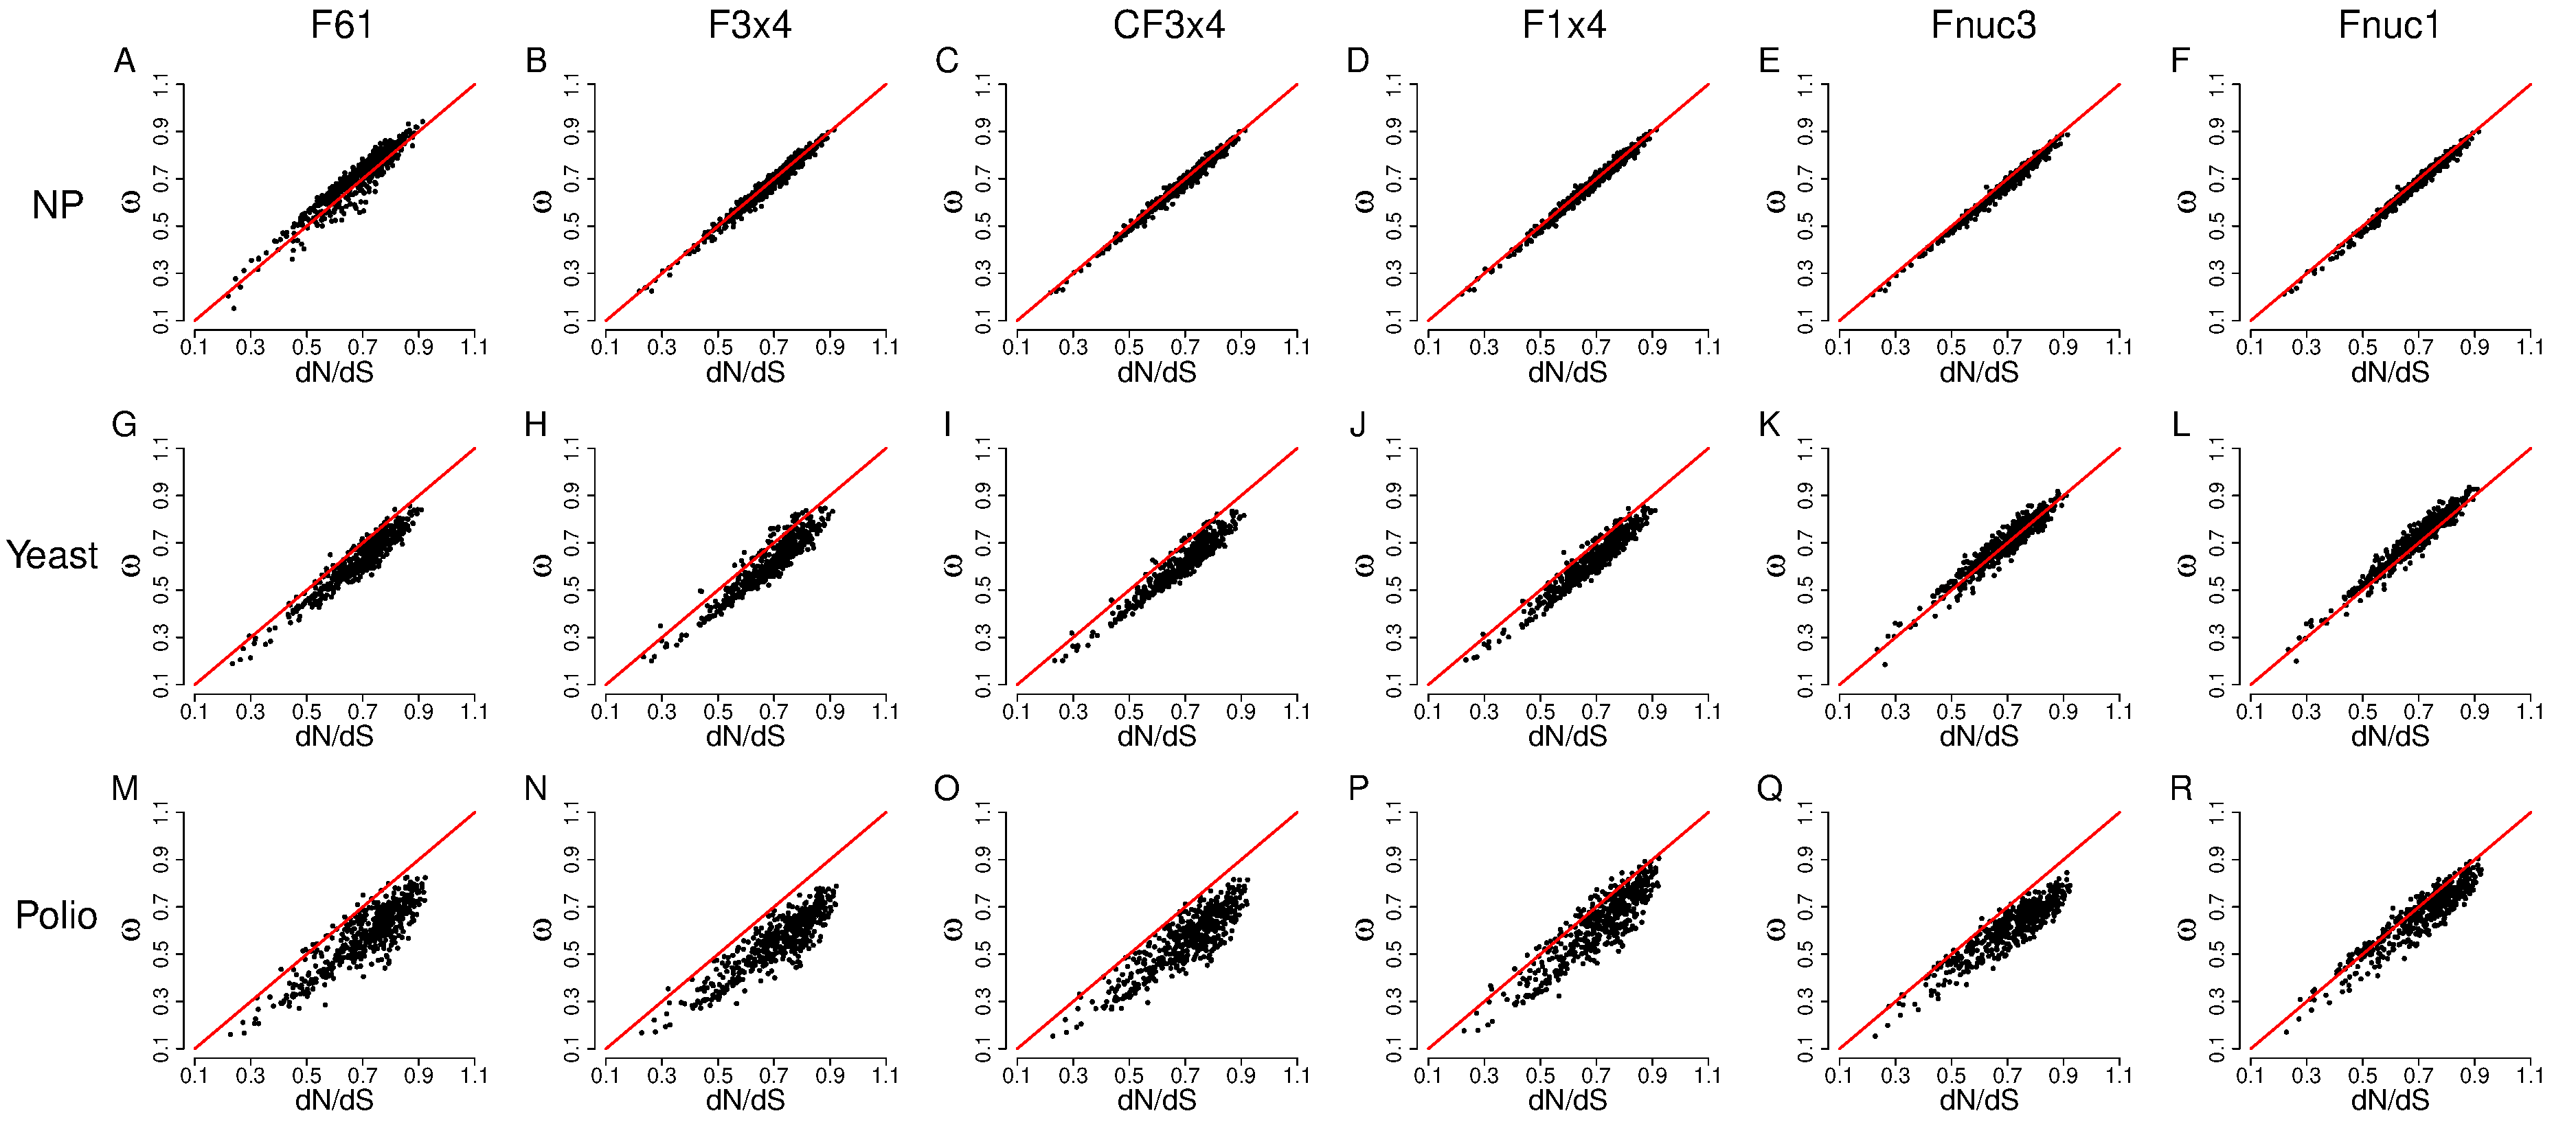
\includegraphics[width=9.5in]{figures/SI/nyp_regression.pdf}
	\vspace{0.5cm}
	
	Figure S1. Regressions of $\omega$ MLEs on the true $dN/dS$ values, as calculated from scaled selection coefficients, for datasets simulated using experimental fitnesses and mutation rates. Each point represents an alignment, and each red line is the $x=y$ line.
\end{landscape}



\end{document}

